\documentclass{article}


\usepackage{authblk}
\usepackage{listings, chngcntr}
\usepackage{textcomp}
\usepackage{float}
\usepackage[T1]{fontenc}
\usepackage{indentfirst}
\usepackage{graphicx}
\usepackage{array}
\usepackage{caption} 
\usepackage{hyperref}
\usepackage{verbatim}
\usepackage{float}
\usepackage{subcaption}
\usepackage{gensymb}
\usepackage{amsmath}
\usepackage{geometry}
\usepackage{multirow}
\usepackage{listings}


\geometry{
    a4paper,
    left=30mm,
    right=30mm,
    top=30mm,
    bottom=40mm
}

\begin{document}

\title{Single Photon Interference}
\author[1]{Woojin Han}
\affil[1]{Seoul National University, Seoul 151-747, Korea}
\maketitle

\begin{abstract}
    In this experiment,

\end{abstract}
\section{Introduction}
 The experiment of light interference is very significant in research of early quantum mechanics.
The interference pattern is used to explain the wave-like nature of light, which is rejected by the photon model.
In this experiment, we checked the light interference pattern in the weak amplitude limits of light, to find the quantum duality of light.
But, the signal is too small and wide variance the statistical method must be checked.
In \ref{intro: data analysis} section, I uploaded to the public the analysis module and the fully activating code.
Secondly, the data points are tightly measured for high trust in the results.

(results)


\subsection{Fitting Functions: Statistical Verification}
\label{intro: statistical_setup_fitting_method}
 The results take the form of two different experimental values, the detector voltage in the laser experiment, and the pulse count data in the single photon limit experiment.
 Firstly, the laser experiment analysis method is described.
 The slit has three different significant values to affect the interference pattern.
 As Fig. \ref{fig: slit_specs}, $\sigma_{1,2}$, the slit width of right, and left in sight of align each respectively. $\Delta$, the distance between two slits.
 For convenient naming to fitting variables, I name the slit specification parameters in the Greek alphabet.
 \begin{figure}[H]
    \centering
    \begin{subfigure}[b]{7cm}
        \centering
        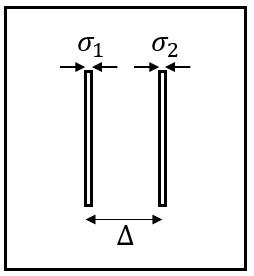
\includegraphics[width=3cm]{../results/slit_specs.png}
        \caption{}
    \end{subfigure}
    \hfill
    \caption{Schematic model of the slit}
    \label{fig: slit_specs}
\end{figure}
 By simple calculations, the double slit results which assume $\sigma1 = \sigma2 = \sigma$ and no spectral dispersion, in each the wavelength of the laser is uniform enough to $\lambda$, follows equation \ref{equation: raw double slit}.
 The fitting parameters are $c, I, d_1, d_2$ which are the center of the detector slit, the center intensity, and the spatial parameters of slit width and distance each.
 Since the values of $\sigma$ and $L$ have an ambiguity of absolute value, only their ratio matters.
 Therefore, I select $d_1, d_2$ instead.


 \begin{align}
     I(x;c,I,d_1,d_2) = &I \left( \frac{\sin(\pi \frac{x-c}{d_1})}{\pi \frac{x-c}{d_1}} \right)^2 (\cos(\pi \frac{x-c}{d_2}))^2  \nonumber \\
     &d_1 = \frac{L \lambda}{\sigma}, \quad d_2 = \frac{L \lambda}{\Delta}  \label{equation: raw double slit}
 \end{align}

 For modeling the dispersed nature of the laser wavelength, the Lorentzian distribution is used.
 Since the laser emits light in band gap resonance, the assumption is valid.
 Equation \ref{equation: double slit light dispersion} shows the Lorentzian profile of the wavelength.
 $\gamma$ is the FWHM value of the wavelength, $\Gamma$ is dimensionless factor of the distribution.
 To detour the ambiguity of $\lambda$ and $\gamma$, I used $\Gamma$ as a fitting parameter.
 $d_i$, the fitting parameters are linear to $\lambda$, the probability density of $d$ while $d_i$ is the central value can be calculated as follows.

 \begin{align}
    &g(\lambda; \gamma) = \frac{1}{\pi} \frac{\frac{\gamma}{2}}{\lambda^2 + (\frac{\gamma}{2})^2} \nonumber \\
    &\gamma = \lambda \times \Gamma \nonumber \\
    &P(d|d_i) = g(\frac{d-d_i}{d_i};\Gamma) \label{equation: double slit light dispersion}
 \end{align}
 
 Finally, the fitting equation is \ref{equation: modified double slit}.
 This type of fitting is written as Laser Broadening Fitting(LBF).
 The integrand function is the simple double-slit function in \ref{equation: raw double slit}.

 \begin{equation}
    I(x;c,I,d_1,d_2,\Gamma) = \int I(x;c,I,d_1(1+\alpha),d_2(1+\alpha),\gamma) g(\alpha;\Gamma) d\alpha
    \label{equation: modified double slit}
 \end{equation}

 In the asymmetric setting in each case of $\sigma_1 \neq \sigma_2$ changes the single slit interference part either.
 But, the condition leads to overfitting since there are too many parameters compared to the data points.
 Therefore, I assume $\sigma_1 \sim \sigma_2$ which gives the difference in the amplitude of light.
 This type of fitting is written as Asymmetric Correction Fitting(ACF).

 \begin{equation}
    I(x;c,I,d_1,d_2, I_2) = \left( \frac{\sin(\pi \frac{x-c}{d_1})}{\pi \frac{x-c}{d_1}} \right)^2 \frac{1}{4}(I + I_2 + 2 \sqrt{I I_2}\cos(2\pi \frac{x-c}{d_2})) 
 \end{equation}
 
 In the laser experiment, many photon limits results are fully explained by those functions.
 But, in the bulb experiment, single photon limit results have different types of measurement occurring.
 The Photomultiplier Tube (PMT) detector amplifies the small size input to the large signal.
 And, the measurement data is the count of the pulse which has the amplified signal over a certain threshold.
 The amplification is controlled by the factor of PMT, High Voltage (HV).
 I assume two things to make a model of PMT pulse count data.
 First, the photon detection probability is uniform of the timescale $1s$.
 Secondly, each photon gives excitation to PMT in uniform amplitude.
 Let single-photon excites the PMT in the amplitude of $V_0$ for $\tau$ seconds.
 And, $n$ number of photons emits in unit time $t_0 >> \tau$ by assumption.
 Then, the probability of the signal $V$, $P(V;j)$ has a relation of equation \ref{equation: PMT}.
 Each photon has the probability to excite the PMT in a certain time for $2\tau/t_0$.
 So, the number of photons follows binomial distribution $B(n,2\tau/t_0)$.
 \begin{equation}
    P(V>(threshold);j) \sim A e^{-2\tau j}
    \label{equation: PMT}
 \end{equation}

 In the definition of $j = n/t_0$, the probability of a pulse count is exponentially related to the input signal.
 By the signal resolution time, the Pulse Counter/Interval Timer(PCIT) value is exponentially dependent on the input signal.
 Moreover, by the assumption of the binomial distribution, the variance of the PCIT value is proportionally linear to the mean value.
 In the fitting of single photon limits, I may check the $1\sigma$ boundary of multiple experiment results, to check the reliability of the fitting method.


 The nonvanishing problem may also be explained by the rejection of the Fraunhofer approximation.
 Those two slit intensities may differ for the distance between two optical routes.
 But this opinion is simply neglected by the precision of this experiment.
 The route distance difference is about $(\frac{\Delta}{L})^2 \sim (\frac{10\mu m}{10 cm})^2 = 10^{-8}$.
 This means that the difference between the route may affect the intensity results, but the effect is negligible with the natural error of $10^{-4}$, voltage measurement.
 Also, the slit size difference $\sigma_1 \neq \sigma_2$ regime is dominating the Fraunhofer correction.
 So, if the fitting function which considers the optical length difference fits well, the fitting data must not be trusted by this p-value test.

 Just like the previous example, the function fits well with many variables.
 Also, there are a lot of parameters in each fitting function, the fitting results may fall into local minima and lose their physical meaning.
 To avoid overfitting, I double-checked the parameters in each fitting method.
 The parameter $c, I,d_i$ must have similar values since they have the physical backgrounds of slit specification.
 If the parameters are significantly different of $2 \sigma$, a p-value of 0.05, I avoid using the fitted results.
 To help the statistical verification, a specially built module is informed at \ref{intro: data analysis}.


 \subsection{Data Analysis Module}
\label{intro: data analysis}
 To fit various functions, the codes are too messy in dealing with data sets.
 Also, the fitting parameters are too many to optimize in strange local minima lots of times.
 The modulation of the initial parameters is not good enough to try in many data sets.
 Therefore, I made the module of fitting and plotting.
 The idea is that the fitting parameters have a relation with the roughly fitted parameters.
 For example, $[c, I,d_1,d_2]$ results in equation \ref{equation: raw double slit} fitting are similar to the results of $[c, I,d_1,d_2,\Gamma]$ in equation \ref{equation: modified double slit}.
 If is not, the physical meaning of each parameter is infringed, which means the results are overfitted.
 Therefore, I made an input of \verb|rough_fitting_functions| and \verb|fitting_param_query| which both take a role in roughly fitting the data itself, to avoid hard manipulation of initial parameters.

 \begin{lstlisting}[language = Python]
    laser_modified_fig = spi.phys_plot(
            data_set_list,
            lambda x: x.parameters,
            lambda x: x.results[0],
            {'align': 3, 'exp_type': 'double_slit'},
            fitting_function= modified_function,
            rough_fitting_functions = [rough_1,fitting_function],
            fitting_param_query = [None,lambda x: [*x[:4],1e-2]],
            p0_function = laser_double_slit_param_setting,
            truncate = lambda x: True if x<0.7 else False,
            export_param_statics = "export.txt"
        )  
 \end{lstlisting}

 For example, above is the example usage of \verb|spi.phys_plot| method.
 The first two inputs are the $x, y$ variables of the plot.
 So, the function will plot the \verb|x.results[0] - x.parameters|.
 I labeled the experiment as align trial 3, the experiment type is double slit.
 And the following \verb|modified_function| is the final fitting equation.
 The \verb|rough_1, fitting_function| are the roughly fitting functions like equation \ref{equation: raw double slit}.
 Sometimes the parameter numbers or the enumerate may change by the functions.
 For example, there are 4 parameters until \verb|fitting_function|, but we need 5 parameters in \verb|modified_function|.
 Then the fitting parameter should follow the query, in this case, \verb|lambda x: [*x[:4],1e-2]| which adds the fifth parameter as $10^{-2}$.
 Moreover, the method exports the parameters in the form of \LaTeX tabular environment in \verb|export_param_statics|.
 The exported example is like \ref{fig: tabular example}.

 \begin{figure}[H]
    \centering
    \begin{tabular}{c|c|c|c}
        \centering
        & & &  \\ \hline 
        1double slit 1& $0.234\pm 1.54e-08$& $0.042\pm 6.522e-06$& 0.9920
    \end{tabular}
    \caption{example output of phys plot method}
    \label{fig: tabular example}
\end{figure}
By using this method, I can fit an enormous amount of data points without wasting time setting initial parameters, or writing the parameters down in the report.
Every code is uploaded in \cite{github}.

\section{Methods}
Apparatus: PMT, PCIT, Oscilloscope, Slits (\cite{spi_spec}).
The slit spacing and its width are published as Fig. \ref{fig: slit_specs_data}.
The laser wavelength is $670 \pm 20 [nm]$, and the bulb interference filter transfers $546 \pm 10 [nm]$ wavelength light in the Lorentzian profile.
The U channel is the main passage of the light, transferring the single slit, double slit, blocker and detector slit in order.
The distance parameter $L, L_0, L_1$ is shown in Fig. \ref{fig: u_channel_specs}, the distance from the double slit to the detector, the distance between the single slit and the double slit, the width between the double slit and the blocker respectively.
$L = 49.81 [cm]$, $L_0 = 32.50 [cm]$, and $L_1 = 0.70 [cm]$ is the measured data of the U channel.

\begin{figure}[H]
    \centering
    \begin{tabular}{  |m{2cm} | m{2.5cm} | m{2.5cm} | m{2.5cm}|  } 
      \hline
      Slit No.& $\Delta [mm]$& $\sigma_1 [mm]$ & $\sigma_2 [mm]$ \\ 
      \hline
      \hline
        14 & $ 0.35 \pm 0.01$& $0.09 \pm 0.01$ & $0.09 \pm 0.01$\\
      \hline
        15 & $ 0.40 \pm 0.01 $& $0.09 \pm 0.01$ & $0.09 \pm 0.01$\\
      \hline
       16 &$ 0.45 \pm 0.01 $& $0.09 \pm 0.01$ & $0.09 \pm 0.01$\\
       \hline

    \end{tabular}
    \caption{Published slit specification data}
    \label{fig: slit_specs_data}
\end{figure}

\begin{figure}[H]
    \centering
    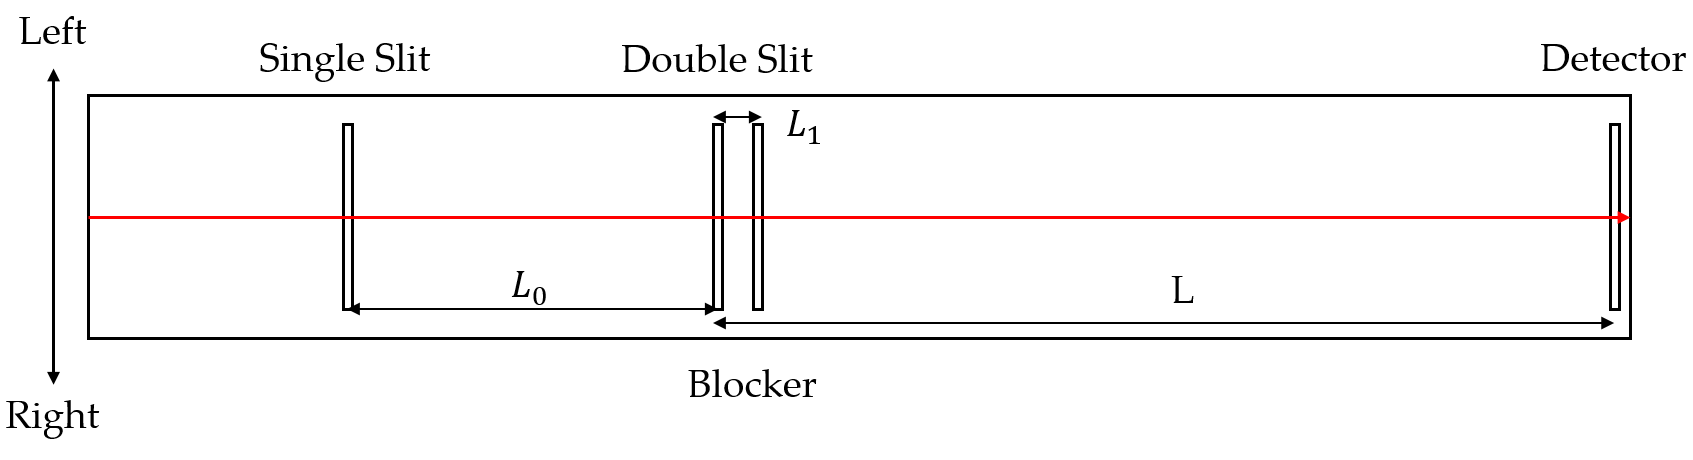
\includegraphics[width=13cm]{../results/u_channel_spec.png}
    \hfill
    \caption{
        Schematic model of U Channel, the laser alignment is represented in the red line, and each slit is plotted in a small box.
        The term left and right definition is also shown.
    }
    \label{fig: u_channel_specs}
\end{figure}
 
\subsection{Laser Experiment}
The multi-photon limit experiment uses the laser as a light source.
The align is fixed for the total measurement, but can not be regenerated.
Therefore, I label the experiment set as aligned number and experiment type.
For each alignment trial, the experiment has done in the double slit, right single slit, and left single slit using a blocker.
For example, in alignment number 1, the double-slit data and the single-slit data are measured.
A total of six alignments are done, in diverse slit conditions.
The data are measured in distance intervals of $0.0025 [cm]$, for $0 - 7 [cm]$. about 300 data points are measured for each experiment type.


\subsection{PMT Threshold}
The PMT have two parameters to control, High Voltage(HV) and the Threshold.
If the HV is too high, the PMT will amplify the dark noise signal into a visible photon signal, which must be avoided.
Besides, if the HV is too low, the PMT will not detect the photon signal and the module have a bad resolution.
The threshold parameter is just the same as negative PMT modulation.
Properly setting the threshold parameter to make PCIT variance low, and setting HV appropriate to the threshold is necessary.
The PMT HV lower boundary is measured in bright conditions.
If the PCIT measurement is not enough visible in the PMT even in the brightest setting, the HV value is not valid.
Also, the PMT HV upper boundary is measured in dark conditions.
If the PCIT measurement is too excited in the PMT even in dark moments, the HV value is not valid.
I have measured 7 times each in 25 different HV values for two different threshold parameter settings.
And the final setting $(HV) = 720 [V], (threshold) = 18.4 [mV]$ has been double-checked with oscilloscope data.

\subsection{Bulb Experiment: Single Photon Limit}
The single-photon limit experiment uses the bulb as a light source.
The alignment is also fixed for the total measurement.
I label the experiment as the aligned number and experiment type and bulb intensity.
For each alignment number, I varied the experiment type in the double, and single slits, and the bulb intensity to 5 from 3, in various slit numbers.
The data are measured 7 times in each position in distance intervals of $0.005 [cm]$, for $0 - 7 [cm]$, about 1500 data points are gathered in each experiment type and bulb intensity.

\section{Results and Discussion}
\subsection{Laser Experiment}

\subsection{PMT Threshold}

\subsection{Bulb Experiment: Single Photon Limit}

\section{Summary}




\bibliography{single_photon_interference_ref}
\bibliographystyle{plain}
\end{document}